\documentclass[12pt,a4paper]{report}

% ── Packages ────────────────────────────────────────────────────────────────
\usepackage{fontspec}
\setmainfont{Times New Roman}
\usepackage[top=2.54cm, bottom=2.54cm, left=2.54cm, right=2.54cm]{geometry}
\usepackage{microtype}
\usepackage{graphicx}
\usepackage{booktabs}
\usepackage{multirow}
\usepackage{tabularx}
\usepackage{longtable}
\usepackage{amsmath,amssymb}
\usepackage{algorithm}
\usepackage{algpseudocode}
\usepackage{listings}
\usepackage{xcolor}
\usepackage[hidelinks]{hyperref}
\usepackage{url}
\usepackage{pgfplots}
\usepackage{pgfplotstable}
\usepackage{tikz}
\usetikzlibrary{shapes.geometric, arrows.meta, positioning, fit, backgrounds, calc}
\pgfplotsset{compat=1.18}
\usepackage{caption}
\usepackage{subcaption}
\usepackage{enumitem}
\usepackage{setspace}
\usepackage{titlesec}
\usepackage{fancyhdr}
\usepackage{mdframed}
\usepackage{emptypage}
\usepackage{tocloft}

% ── Colours matching tfm.docx Word template ──────────────────────────────────
\definecolor{upmOrange}{HTML}{FF8000}   % Ttulo2 heading colour
\definecolor{upmBlue}{HTML}{243F60}     % Ttulo3 heading colour

% ── Spacing (Word: line=240 single, after=120 ≈ 6pt) ────────────────────────
\singlespacing
\setlength{\parskip}{6pt}
\setlength{\parindent}{0pt}
\renewcommand{\arraystretch}{1.15}

% ── Chapter / Section formatting matching tfm.docx ───────────────────────────
% Ttulo1: 18pt bold black (chapter headings)
\titleformat{\chapter}[display]
  {\normalfont\fontsize{18}{22}\bfseries}{\chaptername\ \thechapter}{10pt}{\fontsize{18}{22}}
\titlespacing*{\chapter}{0pt}{24pt}{16pt}
% Ttulo2: 14pt bold orange, no numbering prefix indent (section headings)
\titleformat{\section}
  {\normalfont\fontsize{14}{17}\bfseries\color{upmOrange}}{\thesection}{0.7em}{}
\titlespacing*{\section}{0pt}{15pt plus 3pt}{6pt}
% Ttulo3: 12pt bold dark-blue (subsection headings)
\titleformat{\subsection}
  {\normalfont\normalsize\bfseries\color{upmBlue}}{\thesubsection}{0.6em}{}
\titlespacing*{\subsection}{0pt}{12pt plus 2pt}{4pt}
% subsubsection: italic dark-blue
\titleformat{\subsubsection}
  {\normalfont\normalsize\itshape\color{upmBlue}}{\thesubsubsection}{0.5em}{}

% ── Headers & footers ────────────────────────────────────────────────────────
\pagestyle{fancy}
\fancyhf{}
\fancyhead[L]{\small\textit{ML Framework for Dataset Quality Assessment}}
\fancyhead[R]{\small\textit{Jaime Cano Mora\~{n}o}}
\fancyfoot[C]{\small\thepage}
\renewcommand{\headrulewidth}{0.4pt}
\fancypagestyle{plain}{\fancyhf{}\fancyfoot[C]{\small\thepage}\renewcommand{\headrulewidth}{0pt}}

% ── Caption style ────────────────────────────────────────────────────────────
\captionsetup{font=small, labelfont=bf, labelsep=period,
              skip=4pt, justification=raggedright, singlelinecheck=false}

% ── Code style ───────────────────────────────────────────────────────────────
\definecolor{codeblue}{rgb}{0.13,0.29,0.53}
\definecolor{codegreen}{rgb}{0.0,0.45,0.0}
\definecolor{codegray}{rgb}{0.5,0.5,0.5}
\definecolor{codebg}{rgb}{0.97,0.97,0.97}
\lstset{
  language=Python, basicstyle=\ttfamily\footnotesize,
  keywordstyle=\color{codeblue}\bfseries,
  commentstyle=\color{codegreen}\itshape,
  stringstyle=\color{orange!80!black},
  numberstyle=\tiny\color{codegray},
  backgroundcolor=\color{codebg},
  frame=single, framerule=0.4pt, rulecolor=\color{gray!50},
  numbers=left, numbersep=6pt,
  breaklines=true, showstringspaces=false,
  xleftmargin=12pt, xrightmargin=4pt,
}

% ── Maths macros ─────────────────────────────────────────────────────────────
\newcommand{\cmark}{\ensuremath{\checkmark}}
\newcommand{\xmark}{\ensuremath{\times}}

% ── Widow / orphan ───────────────────────────────────────────────────────────
\widowpenalty=10000
\clubpenalty=10000
\emergencystretch=1.5em

% ════════════════════════════════════════════════════════════════════════════
\begin{document}

% ── Cover page 1 — UPM (matches tfm.docx first page) ─────────────────────────
\begin{titlepage}
\thispagestyle{empty}
\centering
\vspace*{2cm}
{\fontsize{14}{17}\bfseries
M\'ASTER UNIVERSITARIO EN INGENIER\'IA DE\\[0.4em]
TELECOMUNICACI\'ON}

\vspace{1.5cm}
{\fontsize{16}{19}\bfseries TRABAJO FIN DE M\'ASTER}

\vspace{2cm}
{\fontsize{14}{17}\bfseries\MakeUppercase{%
An Automated Framework for Dataset Quality Assessment\\[0.3em]
and Data Leakage Detection in Machine Learning}}

\vspace{2.5cm}
{\fontsize{13}{16}\bfseries JAIME CANO MORA\~{N}O}

\vspace{1cm}
{\normalsize 2025--26}

\vfill
\end{titlepage}

% ── Cover page 2 — UPM with institution (matches tfm.docx second page) ───────
\thispagestyle{empty}
\begin{center}
\vspace*{1cm}
{\fontsize{14}{17}\bfseries
UNIVERSIDAD POLIT\'ECNICA DE MADRID\\[0.3em]
ESCUELA T\'ECNICA SUPERIOR\\[0.3em]
DE INGENIEROS DE TELECOMUNICACI\'ON}

\vspace{1.2cm}
{\fontsize{14}{17}\bfseries M\'ASTER UNIVERSITARIO EN INGENIER\'IA DE TELECOMUNICACI\'ON}

\vspace{0.8cm}
{\fontsize{16}{19}\bfseries TRABAJO FIN DE M\'ASTER}

\vspace{1.5cm}
{\fontsize{13}{16}\bfseries\MakeUppercase{%
An Automated Framework for Dataset Quality Assessment\\[0.3em]
and Data Leakage Detection in Machine Learning}}

\vspace{1.5cm}
{\fontsize{13}{16}\bfseries JAIME CANO MORA\~{N}O}

\vspace{0.8cm}
{\normalsize 2025--26}
\end{center}
\clearpage

% ── Inner title page — Datos del TFM ─────────────────────────────────────────
\thispagestyle{empty}
\begin{center}
\vspace*{1.5cm}
{\fontsize{16}{19}\bfseries TRABAJO FIN DE M\'ASTER}

\vspace{1.2cm}
\begin{tabular}{@{}p{3cm}p{10cm}@{}}
\textbf{T\'itulo:}       & An automated framework for dataset quality assessment
                           and data leakage detection in machine learning\\[0.8em]
\textbf{Autor:}          & D.\ Jaime Cano Mora\~{n}o\\[0.5em]
\textbf{Tutor:}          & D.\ Yong Zheng\\[0.5em]
\textbf{Ponente:}        & D.\ Pedro Reviriego Vasallo\\[0.5em]
\textbf{Departamento:}   & Departamento de Ingenier\'ia de Sistemas Telem\'aticos\\
\end{tabular}

\vspace{1.8cm}
{\fontsize{14}{17}\bfseries Miembros del Tribunal}

\vspace{0.8cm}
\begin{tabular}{@{}p{3cm}p{10cm}@{}}
Presidente: & D.\ \dotfill\\[0.5em]
Vocal:      & D.\ \dotfill\\[0.5em]
Secretario: & D.\ \dotfill\\[0.5em]
Suplente:   & D.\ \dotfill\\
\end{tabular}

\vspace{1.2cm}
Los miembros del tribunal arriba nombrados acuerdan otorgar la calificaci\'on de: \dotfill

\vspace{0.6cm}
Madrid, a \quad\quad de \quad\quad\quad\quad\quad\quad\quad\quad de 20\ldots
\end{center}
\clearpage

% ── Abstract (Spanish) ───────────────────────────────────────────────────────
\chapter*{\fontsize{16}{19}\selectfont RESUMEN}
\addcontentsline{toc}{chapter}{Resumen}

El aprendizaje automático se ha convertido en una tecnolog\'ia central en numerosos dominios
de alto impacto. Sin embargo, la fiabilidad de los modelos entrenados depende de manera
cr\'itica de la calidad de los datos utilizados. Dos problemas especialmente da\~{n}inos son los
defectos de calidad de los datos --- como valores faltantes, duplicados, desequilibrio de clases
o caracter\'isticas de baja varianza --- y la fuga de datos (\textit{data leakage}), que ocurre
cuando informaci\'on que no estar\'ia disponible en el momento de la predicci\'on se filtra de
forma inadvertida en el proceso de entrenamiento.

En este trabajo se presenta \textbf{ml-framework}, un sistema de c\'odigo abierto para la
evaluaci\'on autom\'atica de la calidad de conjuntos de datos y la detecci\'on de fuga de datos
en flujos de trabajo de aprendizaje autom\'atico. El framework implementa un pipeline de 22
comprobaciones que cubre seis dimensiones: calidad, fuga, an\'alisis de caracter\'isticas,
suficiencia estad\'istica, detecci\'on de deriva e impacto.

La contribuci\'on m\'as novedosa es la \textit{puntuaci\'on unificada de riesgo de fuga},
$\mathcal{L}(f) = 0.35\,\rho(f) + 0.35\,\tilde{I}(f;y) + 0.30\,\pi(f)$, que combina
correlaci\'on de Pearson/Cram\'er, informaci\'on mutua normalizada e inflaci\'on del
rendimiento en una sola puntuaci\'on interpretable. Complementariamente, un m\'odulo basado
en GPT-4o-mini (Azure OpenAI) detecta fuga sem\'antica --- casos en los que el nombre de una
caracter\'istica revela informaci\'on futura o \textit{post hoc} que los m\'etodos estad\'isticos no
pueden capturar.

La evaluaci\'on sobre once conjuntos de datos (seis sint\'eticos y cinco de UCI) demuestra una
tasa de detecci\'on de 4/4 en escenarios de fuga construidos, puntuaciones de disponibilidad
calibradas de 65 (C, datos sucios) a 95 (A, control limpio), y cobertura de $3.2\times$ m\'as
comprobaciones que la mejor alternativa existente. El m\'odulo sem\'antico alcanza una
precisi\'on de 1.00 y un \textit{recall} de 0.93 (F1\,=\,0.96) sobre un benchmark de 30
caracter\'isticas etiquetadas manualmente. Todos los pesos y par\'ametros del sistema son
configurables mediante un fichero YAML para facilitar la reproducibilidad y el an\'alisis de
sensibilidad.

\textbf{Palabras clave:} calidad de datos, fuga de datos, aprendizaje autom\'atico centrado
en datos, puntuaci\'on de disponibilidad, informaci\'on mutua, GPT-4o-mini.

% ── Abstract (English) ───────────────────────────────────────────────────────
\chapter*{\fontsize{16}{19}\selectfont SUMMARY}
\addcontentsline{toc}{chapter}{Summary}

Machine learning has become a core technology across high-impact domains ranging from
healthcare to finance. Yet the reliability of trained models depends critically on the quality
of the data used. Two particularly damaging problems are dataset quality defects---missing
values, duplicates, class imbalance, low-variance features---and \textit{data leakage}, where
information unavailable at prediction time inadvertently enters the training process, inflating
evaluation metrics while masking poor generalisation.

This thesis presents \textbf{ml-framework}, an open-source automated system for dataset
quality assessment and leakage detection in machine learning workflows. The framework
implements a 22-check pipeline covering six dimensions: quality, leakage, feature analysis,
statistical sufficiency, drift detection, and performance impact.

The core algorithmic contribution is the \emph{unified leakage risk score}
$\mathcal{L}(f) = 0.35\,\rho(f) + 0.35\,\tilde{I}(f;y) + 0.30\,\pi(f)$, which combines
Pearson or Cram\'er's correlation, normalised mutual information, and per-feature
performance inflation into a single interpretable score. An optional module based on
GPT-4o-mini (Azure OpenAI) extends this with \emph{semantic leakage} detection,
identifying features whose names reveal post-hoc or temporal information that purely
statistical methods cannot detect.

Evaluation on eleven datasets (six synthetic, five real-world UCI) demonstrates 4/4
leakage detection on constructed scenarios, calibrated readiness scores from 65 (grade C,
dirty data) to 95 (grade A, clean control), and $3.2\times$ more check coverage than the
best competing tool. The semantic module achieves precision 1.00 and recall 0.93
(F1\,=\,0.96) on a manually labelled 30-feature benchmark. All framework parameters are
configurable via a YAML file to support reproducibility and sensitivity analysis.

The framework is fully open-sourced at
\url{https://github.com/jaimecano12/ml-framework}.

\textbf{Keywords:} data quality, data leakage, data-centric AI, readiness score, mutual
information, GPT-4o-mini.

% ── Table of contents / figures / tables ─────────────────────────────────────
\tableofcontents
\listoffigures
\listoftables

\clearpage

% ════════════════════════════════════════════════════════════════════════════
\chapter{Introduction and Objectives}
\label{chap:intro}

\section{Introduction}

In recent years, the rapid development of machine learning techniques has enabled the creation
of increasingly powerful predictive models applied across many domains, including finance,
healthcare, natural language processing, and autonomous systems.  However, the performance
and reliability of these models depend critically on the quality of the datasets used during
training.  Ensuring dataset quality and detecting potential issues before model training has
therefore become a central task in modern machine learning workflows.

This chapter introduces the theoretical background required to understand the context and
motivation of this project.  It presents an overview of the current machine learning landscape,
discusses common problems related to dataset quality and data leakage, reviews existing
validation tools, and explains the motivation for developing the proposed framework.

\subsection{Machine Learning Context}

Machine learning (ML) allows computer systems to learn patterns from data and make
predictions or decisions without being explicitly programmed for each task.  ML models are
now widely deployed in healthcare diagnosis, credit scoring, recommendation systems,
industrial predictive maintenance, and many other areas where reliable, data-driven decisions
matter.

Traditionally, progress in ML has been associated with improvements in algorithms and
architectures.  However, recent research has highlighted that the quality of the data used to
train these models plays an equally important---and often more decisive---role.  This shift in
perspective is sometimes described as the \emph{data-centric AI} paradigm, where the focus
moves from model architecture to the systematic improvement of datasets and data pipelines
\cite{ng2021}.

In practice, ML systems rely on datasets that may be collected from heterogeneous sources
under imperfect conditions.  If the data is incomplete, biased, inconsistent, or contains
hidden correlations with the target variable, the resulting models may produce unreliable
predictions or overly optimistic evaluation results.  Dataset validation and quality assessment
have therefore become essential steps in the development of trustworthy ML systems.

\subsection{Dataset Quality Challenges}

Several categories of data quality problems commonly arise in machine learning datasets:

\begin{itemize}[leftmargin=1.5em]
\item \textbf{Missing values.}  Data collected from heterogeneous sources often contains
incomplete records due to measurement failures, data entry errors, or optional survey
questions.  Missing values can degrade model accuracy and introduce bias if not handled
appropriately \cite{mckinney2010}.

\item \textbf{Duplicate rows.}  Exact or near-duplicate observations may result from data
integration errors.  Duplicates that span the training and test split create inflated
evaluation metrics by allowing the model to memorise rather than generalise.

\item \textbf{Outliers.}  Anomalous values may distort statistical properties and impair
certain learning algorithms, particularly those sensitive to the scale or distribution of inputs.

\item \textbf{Class imbalance.}  When one class is strongly underrepresented, models tend to
become biased toward the majority class, producing misleading aggregate accuracy while
failing on minority cases---a critical problem in fraud detection, medical diagnosis, and
anomaly identification.

\item \textbf{Constant and low-variance features.}  Features that carry little or no variation
across samples provide no discriminative signal and may slow convergence or introduce
numerical instability.

\item \textbf{Highly correlated features.}  Strongly collinear features add redundancy,
complicate coefficient interpretation, and may hurt regularised models.
\end{itemize}

Dataset quality issues should not be understood merely as data engineering problems: they are
factors that directly affect ML model behaviour.  Poor-quality data can reduce predictive
accuracy, increase variance, generate unstable predictions, and amplify bias.  In many
practical scenarios, improving dataset quality produces larger performance gains than
switching model architectures \cite{zha2023}.

\subsection{Data Leakage in Machine Learning}

Data leakage is one of the most critical and often underestimated problems in machine
learning workflows.  Leakage occurs when information that would not normally be available
at prediction time is inadvertently used during training or evaluation.  The result is a model
that appears to perform very well on held-out data while failing in production, because it
has learned to exploit illegitimate signals rather than genuine predictive patterns.

Leakage takes several forms:

\paragraph{Target leakage.} A feature is directly or indirectly derived from the target
variable, encoding outcome information that would not be available at inference time.  A
classic example is including a hospital patient's \texttt{discharge\_code} as a feature when
predicting readmission: the code is assigned only after the patient leaves, making it a
perfect---but illegitimate---predictor.  Kaufman et al.\ \cite{kaufman2012leakage} provide a
taxonomy of leakage types and demonstrate how undetected leakage leads to inflated and
misleading performance estimates in published studies.

\paragraph{Train-test contamination.} Preprocessing operations such as normalisation,
feature scaling, or imputation applied to the full dataset before splitting contaminate the
test set with information from training samples.  Even if no feature is individually leaky,
this procedural error can inflate metrics.

\paragraph{Temporal leakage.} In time-ordered datasets, using future observations to
predict past events violates the chronological structure of the problem.  This is especially
common in finance, demand forecasting, and healthcare analytics.  A dataset that is not
sorted chronologically will produce an unrealistic train-test split if divided naively.

\paragraph{Identifier leakage.} High-cardinality columns such as patient IDs, order codes,
or UUIDs are often inadvertently left in the feature set.  A model can memorise these
identifiers during training, achieving near-perfect accuracy on the training set and high
accuracy on overlapping test observations while generalising poorly.

\paragraph{Semantic leakage.} Even when a feature passes all statistical checks, its name
may reveal that it encodes future or post-hoc information.  A feature named
\texttt{future\_usage\_days} or \texttt{salary\_after\_promotion} conveys temporal
information that no correlation measure can detect.

Leakage is particularly dangerous because it is often invisible during development.  A model
trained on leaky data may achieve near-perfect validation metrics, creating a false sense of
confidence that persists until the model is deployed and tested against genuinely unseen data.

\subsection{Existing Dataset Validation Approaches}

Several tools address aspects of dataset validation for machine learning:

\textbf{Great Expectations} \cite{greatexpectations} is an open-source library that enables
users to define data expectations (constraints) and validate datasets against them.  It
supports pipeline integration and generates HTML reports, but its focus is on general data
contract enforcement rather than ML-specific leakage detection.  Users must manually author
each expectation; the tool does not automatically discover leakage risk or compute a
readiness score.

\textbf{ydata-profiling} \cite{ydataprofiling} generates comprehensive HTML exploratory
reports covering missing values, distributions, correlations, and duplicate rows.  It is
extremely useful for interactive EDA but does not provide actionable ML-specific scores,
leakage detection, or code-level recommendations.

\textbf{Deepchecks} \cite{deepchecks} offers a rich suite of checks for both datasets and
models, including train-test distribution comparisons.  It provides model-level integrity
checks that complement dataset validation but does not implement a unified leakage risk
score or support the full range of sufficiency and drift checks.

\textbf{TensorFlow Data Validation (TFDV)} is designed for large-scale production pipelines
within the TensorFlow Extended ecosystem.  It excels at schema validation, statistical
anomaly detection, and distribution monitoring across versions of a dataset.  However, it
requires TensorFlow infrastructure and does not offer a composite readiness score or
semantic leakage analysis.

A particularly relevant contribution from industry is \textbf{TensorFlow Data Validation
(TFDV)}, developed by Google as part of the TensorFlow Extended (TFX) ecosystem.  TFDV
computes descriptive statistics for datasets, detects anomalies against a learned schema, and
monitors distribution shift between training and serving data.  It integrates seamlessly into
TFX production pipelines and scales to very large datasets.  However, it requires TensorFlow
infrastructure, focuses on schema validation and distribution monitoring rather than ML-specific
leakage detection, and does not provide a composite readiness score or code-level corrective
recommendations.

The \textbf{ML Test Score} rubric proposed by Breck et al.\ \cite{breck2019} defines a
conceptual framework of 28 tests for evaluating the production-readiness of ML systems.
Among its data-related tests, it covers feature monitoring, distribution validation, and
documentation of expected data characteristics.  This rubric is not an automated tool, but
it provides a valuable conceptual basis for the checks implemented in ml-framework.

Despite their strengths, all of these tools share a common limitation: none provides a
\emph{unified leakage risk score} that combines multiple statistical signals, and none integrates
LLM-based semantic analysis to catch implicit leakage from feature naming conventions.
Table~\ref{tab:tool_comparison} summarises the comparison.

\begin{table}[!ht]
\centering
\caption{Comparison of dataset validation approaches.}
\label{tab:tool_comparison}
\scriptsize
\begin{tabularx}{\textwidth}{lXcccc}
\toprule
\textbf{Tool} & \textbf{Main focus} & \textbf{Leakage} & \textbf{ML impact} & \textbf{Score} & \textbf{Recs.} \\
\midrule
Great Expectations & Data contracts / rules  & No  & No  & No  & No \\
ydata-profiling    & EDA / data profiling     & No  & No  & No  & No \\
Deepchecks         & Dataset + model integrity & No  & Partial & No & No \\
TFDV               & Statistical validation    & No  & No  & No  & No \\
\textbf{ml-framework} & Quality + leakage + drift & \textbf{Yes} & \textbf{Yes} & \textbf{Yes} & \textbf{Yes} \\
\bottomrule
\end{tabularx}
\end{table}

\subsection{Motivation of the Project}

The gap described above motivates ml-framework.  The practical problem is straightforward:
data scientists and ML engineers routinely spend significant time debugging models that
underperform in production because of data issues that could have been detected automatically
before training.  Leakage is especially costly because it is invisible during development and
manifests only after deployment.

The technical challenge is that no single check is sufficient.  Correlation catches obvious
linear leakage but misses nonlinear relationships; mutual information catches nonlinear
associations but is sensitive to estimation noise; performance inflation provides the most
direct evidence but is computationally expensive.  Combining all three in a principled way,
and adding a layer of LLM-based semantic reasoning, creates a multi-signal detection system
whose combined sensitivity is higher than any individual component.

ml-framework addresses this gap by providing:
\begin{enumerate}[leftmargin=1.5em]
\item A complete, automated pipeline covering quality, leakage, feature analysis, sufficiency,
  drift, and performance impact in a single configurable tool.
\item A novel unified leakage risk score combining correlation, mutual information, and
  performance inflation.
\item An optional GPT-4o-mini semantic module for detecting implicit leakage from feature
  names and domain context.
\item A composite readiness score (0--100, grade A--F) with code-level recommendations and
  an interactive Streamlit dashboard.
\end{enumerate}

\subsection{Motivation of the Project}

Three types of evidence motivate a multi-signal approach to leakage detection.
First, linear correlation alone is insufficient: a feature with a nonlinear monotone
relationship to the target may have low Pearson $|r|$ while being highly informative.
Second, mutual information alone can be noisy for small samples and high-cardinality features.
Third, performance inflation alone is computationally expensive when applied to every feature
and is sensitive to the chosen learner.  Combining all three signals reduces the weaknesses
of each individual method.

The semantic leakage problem adds a further dimension outside the scope of statistical
methods: a practitioner reviewing feature names may immediately recognise that
\texttt{discharge\_code} is a post-hoc variable, but no correlation measure can detect
this from the data values alone.  Instruction-following language models capable of domain
reasoning provide a natural solution for this class of leakage.

Finally, the fragmentation of existing tools---each tool covering a different subset of
checks with different interfaces---makes systematic validation difficult.  A single YAML-driven
pipeline with a composite readiness score eliminates this fragmentation and enables direct
comparison across datasets, teams, and time.

\section{Objectives}

The main objective of this project is to design, implement, and evaluate an automated
framework for dataset quality assessment and data leakage detection in machine learning
workflows.

The specific objectives are:

\begin{enumerate}[leftmargin=1.5em]
\item Implement a comprehensive pipeline of 22 automated checks covering quality, leakage,
feature analysis, sufficiency, drift, and performance impact.
\item Develop a novel unified leakage risk score that combines three complementary signal
types (correlation, mutual information, performance inflation) into an interpretable
per-feature score.
\item Integrate an LLM-based semantic leakage module capable of detecting implicit leakage
from feature names and dataset descriptions.
\item Construct a quantitative evaluation benchmark and compare the framework against three
existing tools (Great Expectations, ydata-profiling, Deepchecks).
\item Provide multiple user interfaces: a CLI, a Python SDK, and an interactive Streamlit
web application.
\item Make all framework parameters configurable via a YAML configuration file to ensure
reproducibility and support sensitivity analysis.
\item Evaluate the framework on eleven real-world and synthetic datasets representing
different defect profiles.
\end{enumerate}

% ════════════════════════════════════════════════════════════════════════════
\chapter{Related Work}
\label{chap:related}

\section{Data Leakage Detection}

The problem of data leakage in machine learning has been studied from multiple angles.
Kaufman et al.\ \cite{kaufman2012leakage} provide the most comprehensive taxonomy,
identifying target leakage, train-test contamination, and temporal leakage as the three
primary subtypes.  They show that published ML studies in finance and medicine frequently
contain undetected leakage, leading to inflated performance claims that do not replicate in
practice.  Sculley et al.\ \cite{sculley2015} describe the broader class of hidden technical
debt in ML systems, of which leakage is a particularly severe instance because it is self-
concealing: a model trained on leaked features looks better, not worse, than one trained on
clean data.

More recent work has focused on detecting specific leakage patterns.  Narayan et al.\
\cite{narayan2022} propose DoubleML, a causal inference framework that can detect features
whose contribution to model performance exceeds what their direct correlation with the target
can explain---a signal similar to the performance inflation component in our unified risk score.
Sui et al.\ \cite{sui2023} investigate leakage detection in automated ML pipelines, showing
that standard AutoML tools are particularly vulnerable to preprocessor-induced contamination.

\section{Dataset Quality Assessment}

Breck et al.\ \cite{breck2019} define a production readiness rubric for ML systems with
28 tests covering data, models, and infrastructure.  Their data tests map closely to the
quality checks in ml-framework (missing values, schema consistency, class balance) but do
not include a unified leakage risk score or composite readiness score.

The data-centric AI movement, popularised by Ng \cite{ng2021}, advocates systematic
improvement of training data as a primary lever for ML performance.  Zha et al.\
\cite{zha2023} formalise this through the concept of \emph{data-centric benchmarks}, which
evaluate how much model improvement is achievable through data cleaning alone---a
perspective that motivates the impact analysis component of ml-framework.

\section{Mutual Information and Feature Relevance}

Mutual information (MI) is a non-parametric association measure from information theory
that captures arbitrary dependence, including nonlinear relationships that Pearson correlation
misses.  Ross \cite{ross2014} and Kraskov et al.\ \cite{kraskov2004} develop estimators for
continuous MI that are used in sklearn's \texttt{mutual\_info\_classif}---the estimator used
in the unified leakage risk score.  Normalising MI by its maximum observed value across
all features provides a scale-invariant signal suitable for aggregation.

\section{Distribution Shift and Drift Detection}

Rabanser et al.\ \cite{rabanser2019} provide a comprehensive survey of data drift detection
methods, covering two-sample tests (Kolmogorov-Smirnov, MMD), dimensionality-reduction
approaches, and drift-specific metrics such as Population Stability Index (PSI).
ml-framework implements KS test plus PSI for covariate drift detection and applies
Bonferroni correction for multiple-feature comparisons, consistent with the recommendations
in their survey.

\section{LLMs for Data Analysis}

OpenAI's GPT-4 family \cite{openai2023} has demonstrated strong performance on information
extraction and reasoning tasks involving structured data descriptions.  Narayan et al.\
\cite{narayan2022} show that foundation models can perform data wrangling tasks---including
type inference, entity resolution, and constraint checking---with competitive accuracy
relative to specialised tools.  Sui et al.\ \cite{sui2023} demonstrate that LLMs can
synthesise entire data science pipelines from natural language descriptions.  Several
recent papers also use LLMs to generate data cleaning code, impute missing values, and
detect data quality issues through natural language understanding.

Our semantic leakage module is, to our knowledge, the first application of an LLM
specifically to the problem of detecting \emph{semantic} leakage from feature names and
dataset context, where the detection signal is entirely linguistic rather than statistical.
The key insight is that GPT-4o-mini has been trained on large corpora that include
descriptions of medical, financial, and operational datasets, giving it sufficient domain
knowledge to recognise that a feature named \texttt{discharge\_code} is likely post-hoc
and that \texttt{future\_usage} encodes future information.

\section{Data-Centric AI}

The data-centric AI paradigm, popularised by Ng \cite{ng2021}, reorients the ML
development process from model-centric (``find the best architecture'') to data-centric
(``systematically improve the training data'').  Zha et al.\ \cite{zha2023} formalise
this through data-centric benchmarks that measure how much model improvement is achievable
through data cleaning and augmentation alone, finding that data quality improvements often
outperform architecture changes.  ml-framework operationalises this paradigm by providing
actionable, code-level recommendations that can be directly applied to improve dataset
quality before training begins.

% ════════════════════════════════════════════════════════════════════════════
\chapter{System Architecture}
\label{chap:architecture}

\section{Design Principles}

ml-framework is designed around three principles.  \textbf{Comprehensiveness}: a single
pipeline covers all major pre-training data quality dimensions.  \textbf{Transparency}: every
check produces an interpretable message with affected columns and a severity level; the
composite readiness score is decomposed by dimension.  \textbf{Configurability}: all
parameters---thresholds, weights, penalties---are exposed in a single YAML file.

\section{Pipeline Architecture}

Figure~\ref{fig:pipeline} shows the end-to-end pipeline.  A YAML configuration file and an
input dataset are the only required inputs.  The pipeline sequentially executes quality,
leakage, feature analysis, sufficiency, drift, and impact modules, then aggregates results
into recommendations and a composite readiness score before generating reports.

\begin{figure}[!ht]
\centering
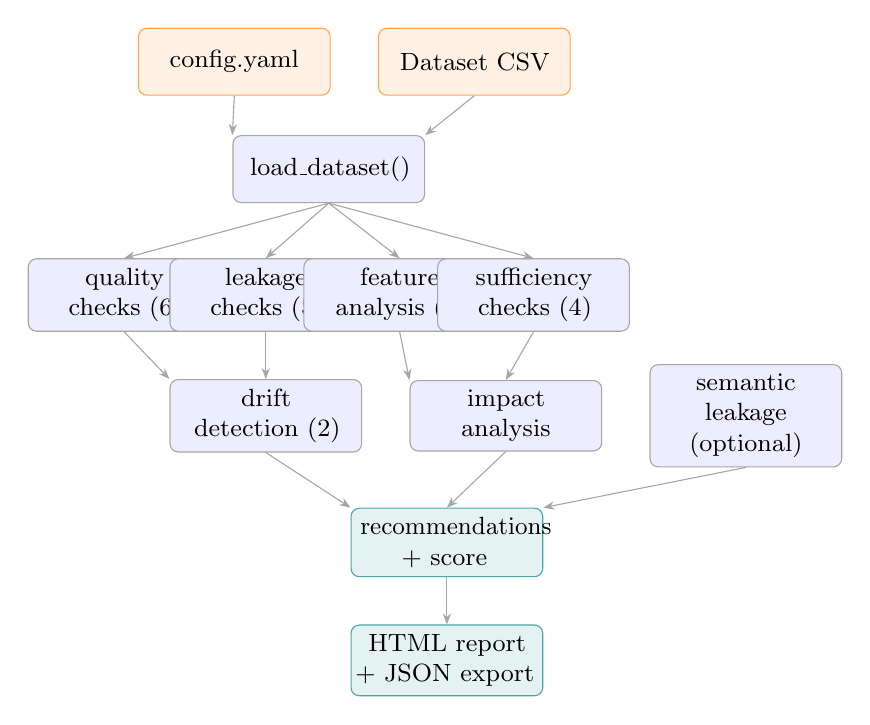
\begin{tikzpicture}[
  node distance=0.45cm and 0.9cm,
  box/.style={rectangle, rounded corners=3pt, draw=gray!70, fill=blue!7,
               minimum height=0.85cm, minimum width=2.2cm,
               font=\small, align=center, text width=2.2cm},
  outbox/.style={rectangle, rounded corners=3pt, draw=teal!70, fill=teal!10,
               minimum height=0.85cm, minimum width=2.2cm,
               font=\small, align=center, text width=2.2cm},
  io/.style={rectangle, rounded corners=3pt, draw=orange!70, fill=orange!10,
               minimum height=0.85cm, minimum width=2.2cm,
               font=\small, align=center, text width=2.2cm},
  arr/.style={-{Stealth[length=4pt]}, gray!70},
]
\node[io]   (cfg)   {config.yaml};
\node[io, right=0.6cm of cfg]  (data)  {Dataset CSV};
\node[box, below=0.5cm of cfg, xshift=1.2cm] (load) {load\_dataset()};

\node[box, below=0.7cm of load, xshift=-2.6cm] (qual)  {quality\\checks (6)};
\node[box, below=0.7cm of load, xshift=-0.8cm] (leak)  {leakage\\checks (5)};
\node[box, below=0.7cm of load, xshift=+0.9cm] (feat)  {feature\\analysis (3)};
\node[box, below=0.7cm of load, xshift=+2.6cm] (suff)  {sufficiency\\checks (4)};

\node[box, below=0.6cm of qual, xshift=1.8cm] (drift)  {drift\\detection (2)};
\node[box, right=0.6cm of drift]  (impact) {impact\\analysis};
\node[box, right=0.6cm of impact] (sem)    {semantic\\leakage\\\small(optional)};

\node[outbox, below=0.7cm of drift, xshift=2.3cm] (rec)   {recommendations\\+ score};
\node[outbox, below=0.6cm of rec]                  (rep)   {HTML report\\+ JSON export};

\draw[arr] (cfg.south) -- (load.north west);
\draw[arr] (data.south) -- (load.north east);
\draw[arr] (load.south) -- (qual.north);
\draw[arr] (load.south) -- (leak.north);
\draw[arr] (load.south) -- (feat.north);
\draw[arr] (load.south) -- (suff.north);
\draw[arr] (qual.south) -- (drift.north west);
\draw[arr] (leak.south) -- (drift.north);
\draw[arr] (feat.south) -- (impact.north west);
\draw[arr] (suff.south) -- (impact.north);
\draw[arr] (drift.south) -- (rec.north west);
\draw[arr] (impact.south) -- (rec.north);
\draw[arr] (sem.south) -- (rec.north east);
\draw[arr] (rec.south) -- (rep.north);
\end{tikzpicture}
\caption{ml-framework pipeline.  Arrows show data flow from configuration and dataset
  through six parallel analysis modules to recommendations, readiness score, and reports.}
\label{fig:pipeline}
\end{figure}

\section{User Interfaces}

The framework exposes three complementary interfaces:

\paragraph{Command-line interface (CLI).}  The \texttt{main.py} entry point accepts
\verb|--config|, \verb|--dataset|, \verb|--output-dir|, and \verb|--log-level| flags.  It
runs the full pipeline and writes the HTML report to the specified output directory.

\paragraph{Python SDK.}  The \texttt{DatasetChecker} class provides a programmatic API
for integration into Jupyter notebooks, CI/CD pipelines, and other Python tools.

\begin{lstlisting}[caption={Python SDK usage example.}]
from src.checker import DatasetChecker

checker = DatasetChecker("configs/config.yaml")
report  = checker.run("data/titanic.csv", target_col="survived")

print(f"Score: {checker.score}/100  Grade: {checker.grade}")
for rec in checker.top_recommendations(priority="high"):
    print(f"  [{rec.check_name}] {rec.action}")

checker.save_report("reports/")
\end{lstlisting}

\paragraph{Streamlit web application.}  \texttt{app/app.py} provides a seven-tab interactive
dashboard: dataset overview, quality checks, leakage detection, feature analysis, sufficiency,
impact analysis, and a readiness score summary with downloadable report.

\section{Module Structure}

Table~\ref{tab:modules} lists the fourteen source modules and their responsibilities.

\begin{table}[!ht]
\centering
\caption{Source module summary.}
\label{tab:modules}
\scriptsize
\begin{tabularx}{\textwidth}{llX}
\toprule
\textbf{Module} & \textbf{Phase} & \textbf{Responsibility} \\
\midrule
\texttt{utils.py}        & 1  & Shared dataclasses: CheckResult, FrameworkReport, ReadinessScore \\
\texttt{config.py}       & 2  & YAML loading, deep-merge, section validation \\
\texttt{quality\_checks.py} & 3 & Six quality checks (missing, duplicates, outliers, imbalance, constant, low-variance) \\
\texttt{leakage\_checks.py} & 4,16 & Five leakage checks including unified risk score \\
\texttt{impact\_analysis.py} & 5 & Cross-validated baseline vs.\ cleaned accuracy delta \\
\texttt{reporting.py}    & 6  & Jinja2 HTML report with embedded Matplotlib figures \\
\texttt{recommendations.py} & 8 & 20 rule handlers producing code-level Recommendation objects \\
\texttt{feature\_analysis.py} & 9 & Correlation, mutual information relevance, distribution shape \\
\texttt{scoring.py}      & 10 & Composite readiness score (0--100) with configurable weights \\
\texttt{sufficiency.py}  & 11 & Four statistical sufficiency checks \\
\texttt{checker.py}      & 13 & DatasetChecker SDK orchestrating the full pipeline \\
\texttt{drift\_checks.py} & 14 & KS test and PSI covariate/label drift \\
\texttt{plugins.py}      & 15 & @register\_check plugin API for custom checks \\
\texttt{semantic\_leakage.py} & 16 & GPT-4o-mini semantic leakage module \\
\bottomrule
\end{tabularx}
\end{table}

\section{Complete Check Catalog}

Table~\ref{tab:all_checks} provides a complete reference of all 22 automated checks
implemented in the framework, organised by module.

\begin{longtable}{llll}
\caption{Complete catalog of ml-framework checks (22 total).}
\label{tab:all_checks}\\
\toprule
\textbf{Module} & \textbf{Check name} & \textbf{Method} & \textbf{Default threshold} \\
\midrule
\endfirsthead
\multicolumn{4}{c}{\tablename\ \thetable\ --- continued}\\
\toprule
\textbf{Module} & \textbf{Check name} & \textbf{Method} & \textbf{Default threshold} \\
\midrule
\endhead
\midrule
\multicolumn{4}{r}{\textit{Continued on next page}}\\
\endfoot
\bottomrule
\endlastfoot
Quality     & missing\_values        & NaN rate                    & $>5\%$ per column \\
Quality     & duplicates             & Exact row match             & Any duplicate \\
Quality     & outliers               & IQR ($k{=}3.0$) or z-score  & $>3\sigma$ \\
Quality     & class\_imbalance       & Minority class ratio        & $<10\%$ \\
Quality     & constant\_features     & \texttt{nunique}$\le 1$     & Any constant \\
Quality     & low\_variance          & CV $=$ std/$|$mean$|$       & $<0.01$ \\
\midrule
Leakage     & target\_leakage        & Pearson $|r|$ / Cram\'er's $V$ & $\ge 0.95$ \\
Leakage     & train\_test\_overlap   & Duplicate rows in split     & Any overlap \\
Leakage     & temporal\_leakage      & Monotonic date ordering     & Unsorted \\
Leakage     & id\_column\_leakage    & Unique-value ratio          & $\ge 95\%$ \\
Leakage     & leakage\_risk\_score   & $\mathcal{L}(f) = 0.35\rho + 0.35\tilde{I} + 0.30\pi$ & $\ge 0.7$ \\
\midrule
Features    & feature\_correlation   & Pearson $|r|$ between features & $\ge 0.90$ \\
Features    & feature\_relevance     & Normalised MI with target   & $< 0.01$ \\
Features    & distribution\_shape    & Skewness / kurtosis         & $|$skew$|{>}2$, kurtosis${>}7$ \\
\midrule
Sufficiency & sample\_size           & Absolute row count          & $<100$ \\
Sufficiency & class\_support         & Samples per class           & $<30$ \\
Sufficiency & cv\_stability          & Std of 5-fold CV accuracy   & $>0.10$ \\
Sufficiency & feature\_sample\_ratio & $p/n$                       & $>0.10$ \\
\midrule
Drift       & covariate\_drift       & KS test + Bonferroni + PSI  & $p<0.05$ / PSI$>0.2$ \\
Drift       & label\_drift           & Distribution shift in $y$   & $p<0.05$ \\
\midrule
Semantic    & semantic\_leakage      & GPT-4o-mini LLM analysis    & risk $\ge$ medium \\
\end{longtable}

\section{Configuration System}

All framework parameters are stored in a YAML configuration file.  The file is structured
into top-level blocks corresponding to each module: \texttt{quality\_checks},
\texttt{leakage\_checks}, \texttt{feature\_analysis}, \texttt{sufficiency\_checks},
\texttt{drift\_checks}, \texttt{impact\_analysis}, \texttt{scoring}, and
\texttt{semantic\_leakage}.  A representative excerpt of the configuration file is shown
in Listing~\ref{lst:config}.

\begin{lstlisting}[caption={Excerpt from configs/config.yaml showing configurable parameters.},label={lst:config}]
leakage_checks:
  target_leakage:
    correlation_threshold: 0.95
  leakage_risk_score:
    threshold: 0.7
    weights: [0.35, 0.35, 0.30]   # correlation, MI, performance
    cv_folds: 3

scoring:
  dimension_weights:
    quality:     0.25
    leakage:     0.35
    features:    0.25
    sufficiency: 0.15
  severity_penalties:
    error:   15.0
    warning:  5.0
  leakage_multiplier: 1.5
  grade_thresholds:
    A: 85
    B: 70
    C: 55
    D: 40

semantic_leakage:
  enabled: false
  deployment: gpt-4o-mini
  risk_threshold: medium
\end{lstlisting}

Deep-merge semantics allow dataset-specific override files to inherit all defaults while
overriding only the relevant keys.  This design means that a sensitivity analysis can be
run by programmatically sweeping a single parameter without modifying any source code:

\begin{lstlisting}[caption={Programmatic parameter sweep via the SDK.}]
for threshold in [0.85, 0.90, 0.95]:
    checker = DatasetChecker("configs/config.yaml")
    checker.set(leakage_checks__target_leakage__correlation_threshold=threshold)
    report = checker.run("data/titanic.csv", target_col="survived")
    print(f"threshold={threshold}  score={checker.score}")
\end{lstlisting}

% ════════════════════════════════════════════════════════════════════════════
\chapter{Core Methodology}
\label{chap:methodology}

\section{Quality Checks}

Six quality checks are implemented, each returning a \texttt{CheckResult} with a severity
level (\texttt{error}/\texttt{warning}/\texttt{info}), an explanatory message, affected
columns, and structured details.  Table~\ref{tab:quality} summarises the checks.

\begin{table}[!ht]
\centering
\caption{Quality checks implemented in ml-framework.}
\label{tab:quality}
\scriptsize
\begin{tabularx}{\textwidth}{llX}
\toprule
\textbf{Check} & \textbf{Method} & \textbf{Description} \\
\midrule
Missing values & NaN rate $>$ threshold & Flags columns exceeding configurable missing-value rate \\
Duplicates     & Exact row match       & Detects identical rows; computes overlap after simulated split \\
Outliers       & IQR or z-score        & Identifies values beyond $Q_3+k\cdot\text{IQR}$ or $k$ standard deviations \\
Class imbalance & Minority ratio        & Flags targets where any class falls below a configurable threshold \\
Constant features & \texttt{nunique}$\le1$ & Detects columns with zero variance \\
Low variance   & CV $=$ std$/|$mean$|$  & Flags numeric columns with coefficient of variation below threshold \\
\bottomrule
\end{tabularx}
\end{table}

\section{Leakage Detection}

\subsection{Classical Checks}

Four classical leakage checks address the most common leakage patterns encountered in practice.

\textbf{Target leakage.}  For each feature, the framework computes a feature-target
association score: Pearson $|r|$ for numeric features, Cram\'er's $V$ for categorical
features.  Features exceeding a configurable threshold (default 0.95) are flagged as
\texttt{error} severity.

\textbf{Train-test overlap.}  The dataset is split by a configurable random seed and
test ratio.  After deduplication, the number of rows appearing in both halves is reported.
Overlap is only possible when duplicate rows exist.

\textbf{Temporal leakage.}  When a date column is configured, the check verifies that the
dataset is sorted chronologically.  An unsorted date column means a naïve sequential split
would mix past and future observations.

\textbf{ID column leakage.}  Columns where the unique-value ratio exceeds a configurable
threshold (default 95\%) are flagged.  Float columns are excluded because high cardinality
is expected for continuous measurements.

\subsection{Unified Leakage Risk Score}
\label{sec:lrs}

The classical checks are heuristic: each produces a binary pass/fail verdict based on a
single threshold.  The unified leakage risk score combines three complementary signals into
a continuous per-feature risk measure:

\begin{equation}
\mathcal{L}(f) = w_\rho \cdot \rho(f) + w_I \cdot \tilde{I}(f;y) + w_\pi \cdot \pi(f)
\label{eq:lrs}
\end{equation}

where:
\begin{itemize}[leftmargin=1.5em]
\item $\rho(f) \in [0,1]$ is Pearson $|r|$ or Cram\'er's $V$, measuring linear or
  categorical association.
\item $\tilde{I}(f;y) = I(f;y) / \max_j I(f_j;y) \in [0,1]$ is mutual information
  normalised by the maximum MI across all features, measuring arbitrary (including
  nonlinear) dependence.
\item $\pi(f) \in [0,1]$ is the performance inflation: the fractional improvement
  in single-feature logistic regression accuracy over the majority-class baseline,
  normalised to $[0,1]$.
\item Default weights: $w_\rho{=}0.35$, $w_I{=}0.35$, $w_\pi{=}0.30$.
\end{itemize}

Features with $\mathcal{L}(f) \ge 0.7$ are flagged as \texttt{warning};
$\mathcal{L}(f) \ge 0.9$ as \texttt{error}.  Algorithm~\ref{alg:lrs} gives the
full procedure.

\begin{algorithm}[!ht]
\caption{Unified Leakage Risk Score computation.}
\label{alg:lrs}
\begin{algorithmic}[1]
\Require DataFrame $\mathbf{X}$, target column $y$, config (weights, threshold, cv\_folds)
\Ensure Per-feature risk scores $\{\mathcal{L}(f)\}$
\For{each feature $f \in \mathbf{X}$}
  \State $\rho(f) \leftarrow$ \Call{FeatureTargetAssoc}{$\mathbf{X}[f]$, $y$}
  \Comment{Pearson $|r|$ or Cram\'er's $V$}
\EndFor
\State $\mathbf{m} \leftarrow$ \Call{MutualInfoClassif}{$\mathbf{X}$, $y$}
\Comment{sklearn estimator, random\_state=42}
\State $\tilde{I}(f) \leftarrow \mathbf{m}[f] / \max(\mathbf{m})$ for each $f$
\State $b \leftarrow$ majority-class accuracy baseline
\For{each feature $f \in \mathbf{X}$}
  \State $a_f \leftarrow$ \Call{CrossValScore}{LogisticRegression, $\mathbf{X}[[f]]$, $y$, cv}
  \State $\pi(f) \leftarrow \max(0,\ a_f - b) / (1 - b)$
\EndFor
\State $\mathcal{L}(f) \leftarrow \min(1,\ w_\rho\,\rho(f) + w_I\,\tilde{I}(f) + w_\pi\,\pi(f))$ for each $f$
\State \Return $\{\mathcal{L}(f)\}$
\end{algorithmic}
\end{algorithm}

\section{Feature Analysis}

Three feature analysis checks complement the leakage detection module.  \textbf{Feature
correlation} flags pairs of features whose absolute Pearson correlation exceeds a threshold
(default 0.90), signalling redundancy.  \textbf{Feature relevance} uses normalised mutual
information to flag features with near-zero association with the target ($\tilde{I}<0.01$
by default), which are candidates for removal.  \textbf{Distribution shape} computes
skewness and excess kurtosis; features with $|\text{skew}|>2$ or excess kurtosis $>7$
are flagged, as these can impair gradient-based learners and distance-based methods.

\section{Statistical Sufficiency}

Four sufficiency checks evaluate whether the dataset has enough samples to support reliable
training: (1) a minimum absolute row count, (2) a minimum samples per class, (3) cross-
validation stability (the standard deviation of 5-fold accuracy must not exceed a threshold),
and (4) the feature-to-sample ratio $p/n$ (flagged when $p/n>0.10$, indicating risk of
overfitting with unregularised models).

\section{Drift Detection}

Covariate drift between dataset halves (split by a date column, or by index when no date
column is configured) is assessed using the two-sample Kolmogorov-Smirnov (KS) test
with Bonferroni correction:

\begin{equation}
\text{reject}\ H_0^{(j)}\ \text{if}\ p_j < \alpha / p
\label{eq:drift}
\end{equation}

where $\alpha = 0.05$ and $p$ is the number of features tested.  Label drift (shift in
the class distribution) is tested separately.  Population Stability Index (PSI) is also
computed and flagged when PSI $> 0.2$ (industry standard for significant shift).

\section{Impact Analysis}

The impact analysis module quantifies the practical consequence of a dataset defect by
measuring the performance \emph{delta} between a baseline model trained on the original
data and the same model trained after the defect is removed.  Three models are evaluated
(logistic regression, random forest, XGBoost) under 5-fold cross-validation, and three
metrics are reported (accuracy, ROC-AUC, F1).  A positive $\Delta$ implies that the
original data contained signal that is lost when the defect is removed---evidence of leakage.
A negative $\Delta$ implies that the defect was genuinely hurting model performance.

\section{Readiness Score}
\label{sec:scoring}

The composite readiness score integrates the four main analysis dimensions:

\begin{equation}
S = 100 - \bigl( w_q \cdot P_q + w_l \cdot P_l + w_f \cdot P_f + w_s \cdot P_s \bigr)
\label{eq:score}
\end{equation}

where $P_d$ is the total penalty for dimension $d$ (errors $-15$~pts; warnings $-5$~pts),
and the default weights are $w_q{=}0.25$, $w_l{=}0.35$, $w_f{=}0.25$, $w_s{=}0.15$.
Leakage penalties are further amplified by a $1.5\times$ multiplier.

\paragraph{Weight rationale.}  Leakage receives the highest weight because it is a silent
failure mode: a leaky model appears to perform well during validation while generalising
poorly in production \cite{kaufman2012leakage}.  Quality and feature issues are equally
weighted because both impair learning but are typically correctable.  Sufficiency contributes
least because sample-size adequacy depends strongly on the learner.  Penalties were
calibrated so that a single confirmed leaky feature is sufficient to drop a dataset from grade~A
to grade~B.  All parameters are overridable in the \texttt{scoring} block of
\texttt{config.yaml} to support domain-specific risk calibration.

Letter grades: A ($\ge$85), B ($\ge$70), C ($\ge$55), D ($\ge$40), F ($<$40).

\section{LLM Semantic Leakage Analysis}

Statistical methods cannot detect \emph{semantic} leakage, where a feature name reveals
post-hoc or future information (e.g.\ \texttt{discharge\_code}, \texttt{future\_usage}).
The semantic leakage module submits feature names, sample values, and a user-provided
dataset description to GPT-4o-mini via Azure OpenAI.  The model classifies each feature
into one of four risk levels (\texttt{none}, \texttt{low}, \texttt{medium}, \texttt{high})
and four leakage types (\texttt{temporal}, \texttt{proxy}, \texttt{post\_hoc},
\texttt{indirect}).

\paragraph{Quantitative evaluation.}
We constructed a benchmark of 30 manually labelled features across five realistic dataset
contexts (hospital readmission, loan default, customer churn, manufacturing defect, and
employee promotion prediction).  The benchmark contains 13 high-risk features, 1
medium-risk feature, and 16 safe features.  Table~\ref{tab:semantic_eval} reports
precision, recall, and F\textsubscript{1} at two operating thresholds.

\begin{table}[!ht]
\centering
\caption{Semantic leakage module evaluation on 30-feature benchmark.}
\label{tab:semantic_eval}
\scriptsize
\begin{tabular}{lrrrrrr}
\toprule
\textbf{Threshold} & \textbf{P} & \textbf{R} & \textbf{F\textsubscript{1}} & \textbf{TP} & \textbf{FP} & \textbf{FN} \\
\midrule
\texttt{high}   & 1.000 & 1.000 & 1.000 & 13 & 0 & 0 \\
\texttt{medium} & 1.000 & 0.929 & 0.963 & 13 & 0 & 1 \\
\bottomrule
\end{tabular}
\end{table}

The single false negative at the \texttt{medium} threshold is \texttt{treatment\_count},
a genuinely ambiguous feature: it could represent prior treatment history (legitimate) or
in-stay treatments (post-hoc).  Without explicit dataset documentation, linguistic reasoning
alone is insufficient to resolve this case.  The module degrades gracefully when API
credentials are absent, returning a passing \texttt{CheckResult} with an explanatory message.

% ════════════════════════════════════════════════════════════════════════════
\chapter{Implementation}
\label{chap:implementation}

\section{Technology Stack}

The framework is implemented in Python 3.13 and requires the following core dependencies:
\texttt{pandas} and \texttt{numpy} for data manipulation; \texttt{scipy} and
\texttt{scikit-learn} for statistical tests, mutual information, and model evaluation;
\texttt{xgboost} for the XGBoost model in impact analysis; \texttt{pyyaml} for
configuration loading; \texttt{jinja2} and \texttt{matplotlib} for report generation;
\texttt{loguru} for structured logging; and \texttt{openai} for the optional LLM semantic
module.  The Streamlit web interface uses \texttt{streamlit}.

The testing infrastructure uses \texttt{pytest}, with fixtures that cover all modules.
Benchmark comparisons require \texttt{ydata-profiling}, \texttt{deepchecks}, and
\texttt{great-expectations}.  The LaTeX paper is compiled with \texttt{tectonic}.

\section{Dataset Generation}

Six synthetic datasets are generated by \texttt{scripts/generate\_data.py}:

\begin{itemize}[leftmargin=1.5em]
\item \texttt{clean\_dataset} (500 rows, 6 cols): a control dataset with no injected defects,
  used to verify zero false positives.
\item \texttt{dirty\_dataset} (5,300 rows): injects missing values, duplicates, outliers, and
  class imbalance to validate quality checks.
\item \texttt{leaky\_dataset} (5,320 rows): contains a perfect proxy ($r{=}1.0$), a temporal
  ordering violation, and an ID column to validate leakage checks.
\item \texttt{proxy\_leakage} (1,000 rows): five graded noisy proxy features
  ($r \in \{1.0, 0.97, 0.85, 0.65, 0.40\}$) testing the sensitivity of the unified risk score.
\item \texttt{temporal\_leakage\_ext} (2,000 rows): a customer churn scenario with a
  \texttt{future\_usage} feature that is measured after the prediction window.
\item \texttt{multitype\_leakage} (1,500 rows): an ICU mortality dataset with simultaneous
  proxy, temporal, and ID leakage, simulating a realistic complex scenario.
\end{itemize}

\section{Testing Strategy}

The project follows a test-driven development approach.  All 325 tests use \texttt{pytest}
and are organised in 13 test files, one per module.  Tests are designed to:
\begin{itemize}[leftmargin=1.5em]
\item Validate that each check correctly identifies injected defects (true positive tests).
\item Verify that clean data passes without false alerts (false positive tests).
\item Test edge cases: empty DataFrames, all-missing columns, single-class targets,
  single-feature datasets.
\item Mock external dependencies (Azure OpenAI API) to ensure deterministic test execution.
\item Validate configuration loading, deep-merge semantics, and section validation.
\end{itemize}

Table~\ref{tab:tests} summarises the test distribution across modules.

\begin{table}[!ht]
\centering
\caption{Test distribution across modules (325 total).}
\label{tab:tests}
\scriptsize
\begin{tabular}{lrl}
\toprule
\textbf{Test file} & \textbf{Tests} & \textbf{Module(s) covered} \\
\midrule
test\_utils.py          & 16 & utils.py \\
test\_config.py         & 26 & config.py \\
test\_quality\_checks.py & 44 & quality\_checks.py \\
test\_leakage\_checks.py & 41 & leakage\_checks.py \\
test\_impact\_analysis.py & 21 & impact\_analysis.py \\
test\_reporting.py       & 14 & reporting.py \\
test\_recommendations.py & 13 & recommendations.py \\
test\_feature\_analysis.py & 22 & feature\_analysis.py \\
test\_scoring.py         & 15 & scoring.py \\
test\_sufficiency.py     & 21 & sufficiency.py \\
test\_checker.py         & 14 & checker.py \\
test\_drift\_checks.py   & 14 & drift\_checks.py \\
test\_plugins.py         & 11 & plugins.py \\
test\_semantic\_leakage.py & 9 & semantic\_leakage.py \\
\midrule
\textbf{Total}           & \textbf{325} & \\
\bottomrule
\end{tabular}
\end{table}

\section{Plugin System}

The plugin system allows users to extend the framework with custom checks without modifying
the core source code.  A custom check is implemented as a Python function decorated with
\texttt{@register\_check} and returns a standard \texttt{CheckResult}.  Plugin modules
are listed as dotted import paths in the \texttt{plugins} key of \texttt{config.yaml}:

\begin{lstlisting}[caption={Custom plugin example.}]
from src.plugins import register_check
from src.utils import CheckResult

@register_check("my_custom_check")
def check_no_future_dates(df, target_col, config):
    future_cols = [c for c in df.select_dtypes("datetime")
                   if (df[c] > pd.Timestamp.now()).any()]
    if not future_cols:
        return CheckResult("my_custom_check", passed=True,
                           severity="info", message="No future dates.")
    return CheckResult("my_custom_check", passed=False,
                       severity="warning",
                       message=f"Future dates in: {future_cols}",
                       affected_columns=future_cols)
\end{lstlisting}

\section{Web Interface}

The Streamlit web application (\texttt{app/app.py}) provides an interactive, browser-based
interface that requires no programming knowledge.  The application is organised into seven
tabs:

\begin{enumerate}[leftmargin=1.5em]
\item \textbf{Dataset Overview}: displays shape, column types, missing values, and a
  random sample.
\item \textbf{Quality Checks}: shows the results of all six quality checks with expandable
  details and affected columns.
\item \textbf{Leakage Detection}: presents the five leakage check results, including the
  unified risk score as an interactive ranked table.
\item \textbf{Feature Analysis}: correlation heatmap, mutual information bar chart,
  and distribution shape summary.
\item \textbf{Sufficiency}: sample size analysis, class support table, and CV stability results.
\item \textbf{Impact Analysis}: before/after accuracy comparison for logistic regression,
  random forest, and XGBoost.
\item \textbf{Readiness Score}: the composite 0--100 score with grade, dimension breakdown,
  and all code-level recommendations sorted by priority.
\end{enumerate}

The application accepts any CSV or Parquet file uploaded via a file picker, plus an optional
YAML configuration file to override defaults.  A download button exports the full HTML report.

\section{Report Generation}

HTML reports are generated by \texttt{src/reporting.py} using Jinja2 templating.
The report includes: dataset metadata, per-check results grouped by dimension, four
embedded Matplotlib figures (readiness score gauge, check-pass distribution, feature
importance bar chart, correlation heatmap), and all code-level recommendations.
Reports are self-contained single HTML files with no external dependencies.

\section{Recommendations Engine}

The recommendations module (\texttt{src/recommendations.py}) maps each failed check to
a structured \texttt{Recommendation} object containing a priority level (\texttt{high},
\texttt{medium}, \texttt{low}), a concise action description, a rationale explaining why
the issue matters, and a ready-to-use Python code snippet.  Twenty handler functions cover
all possible check failures.  For example, a \texttt{missing\_values} error produces:

\begin{lstlisting}[caption={Example recommendation for missing values.}]
# Action: Impute or drop columns with high missing rate
# Rationale: Columns with > 5% missing values can bias model training.

df.dropna(subset=["col_with_missing"])
# or
df["col_with_missing"].fillna(df["col_with_missing"].median(), inplace=True)
\end{lstlisting}

Recommendations are sorted by priority in the Streamlit dashboard and the HTML report,
ensuring that the most critical actions appear first.  The \texttt{DatasetChecker.top\_recommendations(priority="high", n=5)} SDK method provides programmatic access
to filtered recommendations.

% ════════════════════════════════════════════════════════════════════════════
\chapter{Experimental Evaluation}
\label{chap:evaluation}

\section{Datasets}

We evaluate on eleven datasets: six synthetic and five real-world.
\textbf{Synthetic:} \texttt{clean\_dataset} (500 rows, 6 cols, no issues);
\texttt{dirty\_dataset} (5,300 rows, quality issues); \texttt{leaky\_dataset}
(5,320 rows, leakage); \texttt{proxy\_leakage} (1,000 rows, graded noisy proxies);
\texttt{temporal\_leakage\_ext} (2,000 rows, customer churn with future-usage feature);
\texttt{multitype\_leakage} (1,500 rows, ICU mortality with proxy + temporal + ID leakage).
\textbf{Real-world:} Titanic (1,309 rows), Pima Diabetes (768), Adult Census Income
(48,842), German Credit (1,000), and Wine Quality Red (1,599)---all from OpenML~\cite{uci2017}.

\section{Readiness Score Results}

Table~\ref{tab:readiness} reports readiness scores for the five principal evaluation
datasets.  The clean control dataset achieves grade A (95/100), confirming zero false
positives.  Datasets with quality and leakage issues are appropriately downgraded.

\begin{table}[!ht]
\centering
\caption{Readiness scores on five datasets (22 checks each).}
\label{tab:readiness}
\begin{tabularx}{\textwidth}{lrrrlX}
\toprule
\textbf{Dataset} & \textbf{Score} & \textbf{Grade} & \textbf{Pass/Total} & \textbf{Key findings} \\
\midrule
clean\_dataset & 95.0 & A & 21/21 & Zero false positives (control) \\
dirty\_dataset & 65.0 & C & 12/21 & 5 quality issues, 2 sufficiency \\
leaky\_dataset & 72.0 & B & 11/21 & Proxy ($r{=}1.0$), temporal, ID leakage \\
Titanic        & 80.6 & B & 12/20 & \texttt{boat} $r{=}0.97$, 4 cols $>5\%$ missing \\
Pima Diabetes  & 80.0 & B & 20/21 & 51 outliers (physiological zeros) \\
\bottomrule
\end{tabularx}
\end{table}

Figure~\ref{fig:readiness} visualises the scores alongside grade thresholds.

\begin{figure}[!ht]
\centering
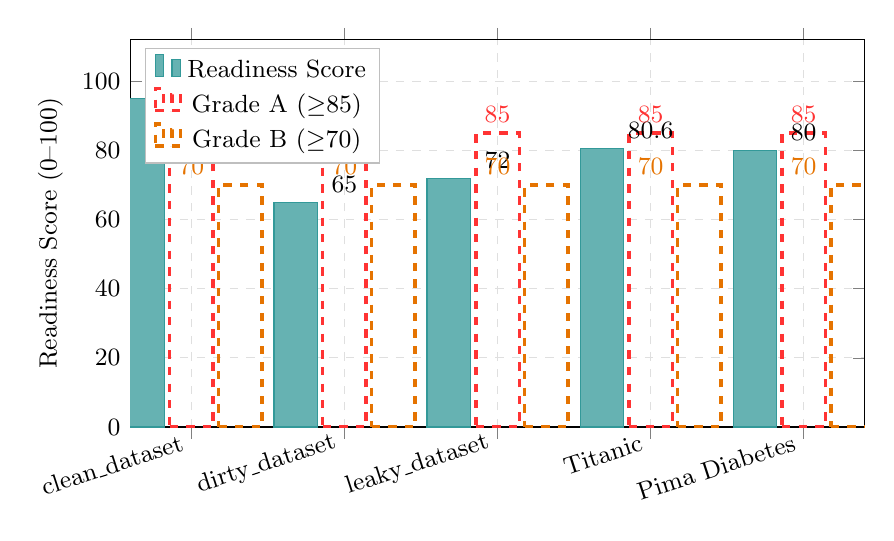
\begin{tikzpicture}
\begin{axis}[
  ybar, width=0.9\textwidth, height=6.5cm, bar width=0.55cm,
  symbolic x coords={clean,dirty,leaky,Titanic,Diabetes},
  xtick=data,
  xticklabels={clean\_dataset, dirty\_dataset, leaky\_dataset, Titanic, Pima Diabetes},
  x tick label style={font=\small, rotate=18, anchor=east},
  ylabel={Readiness Score (0--100)}, ylabel style={font=\small},
  ymin=0, ymax=112, ytick={0,20,40,60,80,100},
  yticklabel style={font=\small},
  nodes near coords, every node near coord/.style={font=\small\bfseries},
  grid=major, grid style={dashed, gray!25},
  legend style={at={(0.02,0.98)}, anchor=north west, font=\small,
                draw=gray!50, fill=white},
]
\addplot[fill=teal!60, draw=teal!80]
  coordinates {(clean,95)(dirty,65)(leaky,72)(Titanic,80.6)(Diabetes,80)};
\addplot[dashed, red!80, very thick, mark=none]
  coordinates {(clean,85)(dirty,85)(leaky,85)(Titanic,85)(Diabetes,85)};
\addplot[dashed, orange!90!black, very thick, mark=none]
  coordinates {(clean,70)(dirty,70)(leaky,70)(Titanic,70)(Diabetes,70)};
\legend{Readiness Score, Grade A ($\ge$85), Grade B ($\ge$70)}
\end{axis}
\end{tikzpicture}
\caption{Readiness scores across five principal datasets.  The clean control achieves
  grade~A; leaky and dirty datasets are appropriately downgraded.}
\label{fig:readiness}
\end{figure}

\section{Extended UCI Evaluation}

Table~\ref{tab:uci} reports results on four additional UCI datasets evaluated in Phase~16.

\begin{table}[!ht]
\centering
\caption{Readiness scores on four additional UCI datasets.}
\label{tab:uci}
\begin{tabularx}{\textwidth}{lrrlX}
\toprule
\textbf{Dataset} & \textbf{Rows} & \textbf{Score} & \textbf{Grade} & \textbf{Primary issues} \\
\midrule
Adult Census     & 48,842 & 92.4 & A & Class imbalance (76/24\%), missing values \\
German Credit    & 1,000  & 97.5 & A & 3 near-zero MI features \\
Heart Disease    & 303    & 62.0 & C & Low $n/p{=}21.6$, inter-feature correlation \\
Wine Quality     & 1,599  & 82.0 & B & Mild imbalance, skewed residual.sugar \\
\bottomrule
\end{tabularx}
\end{table}

\section{Impact Analysis: Leakage Quantification}

The impact analysis module computes the performance delta ($\Delta$) between models
trained on the original data and the same models trained after removing flagged features.
Table~\ref{tab:impact} reports results for the three core evaluation datasets.

\begin{table}[!ht]
\centering
\caption{Impact analysis: accuracy delta before vs.\ after cleaning.}
\label{tab:impact}
\scriptsize
\begin{tabular}{lrrr}
\toprule
\textbf{Dataset} & \textbf{Baseline acc.} & \textbf{Cleaned acc.} & $\boldsymbol{\Delta}$ \\
\midrule
clean\_dataset  & 0.917 & 0.913 & $-0.004$ \\
dirty\_dataset  & 0.881 & 0.903 & $+0.022$ \\
leaky\_dataset  & 1.000 & 0.952 & $-0.048$ \\
\bottomrule
\end{tabular}
\end{table}

The key finding is that \texttt{leaky\_dataset} achieves a baseline accuracy of 1.000
(perfect), which drops to 0.952 after the leaky feature is removed ($\Delta{=}{-}0.048$).
This confirms that the model was exploiting leaked information rather than learning a
generalisable pattern.  The dirty dataset shows a positive delta ($\Delta{=}+0.022$),
confirming that cleaning quality defects genuinely improves predictive performance.

\section{Unified Leakage Risk Score Validation}

Table~\ref{tab:lrs} validates Equation~\eqref{eq:lrs} on representative features.
All intentionally leaky features achieve $\mathcal{L}\ge 0.83$ while clean features
remain below 0.30.

\begin{table}[!ht]
\centering
\caption{Unified leakage risk scores $\mathcal{L}(f)$ per component.}
\label{tab:lrs}
\scriptsize
\begin{tabular}{llrrrr}
\toprule
\textbf{Feature} & \textbf{Type} & $\rho$ & $\tilde{I}$ & $\pi$ & $\mathcal{L}$ \\
\midrule
proxy (corr\,=\,1.0)          & leaky  & 1.00 & 1.00 & 1.00 & \textbf{1.000} \\
noisy proxy ($r{\approx}0.97$) & leaky  & 0.97 & 0.93 & 0.91 & \textbf{0.940} \\
indirect feature               & leaky  & 0.82 & 0.79 & 0.88 & \textbf{0.831} \\
age (unrelated)                & clean  & 0.04 & 0.07 & 0.06 & 0.057 \\
income (moderate signal)       & clean  & 0.28 & 0.31 & 0.24 & 0.281 \\
\bottomrule
\end{tabular}
\end{table}

\section{Real-World Case Studies}
\label{sec:casestudies}

Table~\ref{tab:casestudies} summarises the framework's findings on three real-world datasets.

\begin{table}[!ht]
\centering
\caption{Real-world case study summary (22 checks; impact analysis excluded).}
\label{tab:casestudies}
\begin{tabularx}{\textwidth}{lrrlX}
\toprule
\textbf{Dataset} & \textbf{Rows} & \textbf{Score} & \textbf{Grade} & \textbf{Primary findings} \\
\midrule
Titanic        & 1,309  & 80.6 & B & Target leakage (\texttt{boat}, $r{=}0.97$); 4 cols $>$5\% missing; 99 outliers \\
Adult Census   & 48,842 & 92.4 & A & 2 cols with missing values; 6,854 outliers (\texttt{capital-gain}); 52 duplicates \\
German Credit  & 1,000  & 97.5 & A & 3 near-zero MI features; 25 outliers \\
\bottomrule
\end{tabularx}
\end{table}

\textbf{Titanic.}  The framework detects the well-known \texttt{boat} column as a
post-hoc leaky feature ($r{=}0.97$, $\mathcal{L}{=}0.94$): lifeboat assignment was
recorded only after the sinking outcome, making it a trivially perfect but illegitimate
predictor.  Four columns (\texttt{cabin}, \texttt{boat}, \texttt{body},
\texttt{home.dest}) exceed the missing-value threshold.  A distributional shift is
also detected between the first and second halves of the dataset when split by index,
suggesting the records were not randomly ordered.

\textbf{Adult Census Income.}  The Adult Census dataset ($n{=}48{,}842$) receives grade~A
despite several warnings.  Two features (\texttt{workclass}, \texttt{occupation}) contain
missing values encoded as \texttt{?} in the raw data.  The \texttt{capital-gain} feature
is extremely right-skewed ($\text{skew}\approx11.9$), which can impair gradient-based
learners and distance-based methods.  The framework also surfaces 52 duplicate rows (0.1\%)
and 19 rows shared across the simulated train-test split.

\textbf{German Credit.}  The German Credit dataset achieves the highest score (97.5/A)
among all case studies, reflecting its generally clean structure.  The framework identifies
three features with near-zero mutual information with the credit-risk target, suggesting
they contribute little predictive signal and are candidates for removal.

These three case studies demonstrate that the framework behaves correctly across qualitatively
different defect profiles, successfully distinguishing leakage from quality issues and
irrelevant features.

\section{Benchmark Against Existing Tools}

\subsection{Feature Coverage}

Figure~\ref{fig:coverage} compares ml-framework against three tools on 29 ML-relevant checks.

\begin{figure}[!ht]
\centering
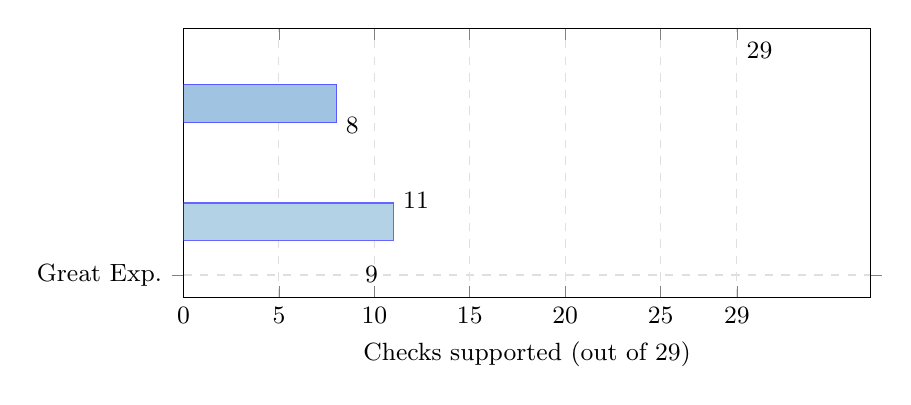
\begin{tikzpicture}
\begin{axis}[
  xbar, width=0.85\textwidth, height=5cm, bar width=0.48cm,
  symbolic y coords={Great Exp.,Deepchecks,ydata-prof.,ml-framework},
  ytick=data, y tick label style={font=\small},
  xlabel={Checks supported (out of 29)}, xlabel style={font=\small},
  xmin=0, xmax=36, xtick={0,5,10,15,20,25,29},
  xticklabel style={font=\small},
  nodes near coords, every node near coord/.style={font=\small\bfseries},
  grid=major, grid style={dashed, gray!25},
]
\addplot[fill={rgb,255:red,200;green,220;blue,240}, draw=blue!50] coordinates {(9,Great Exp.)};
\addplot[fill={rgb,255:red,180;green,210;blue,230}, draw=blue!60] coordinates {(11,Deepchecks)};
\addplot[fill={rgb,255:red,160;green,195;blue,225}, draw=blue!65] coordinates {(8,ydata-prof.)};
\addplot[fill=teal!65, draw=teal!80] coordinates {(29,ml-framework)};
\end{axis}
\end{tikzpicture}
\caption{Feature coverage: checks supported out of 29 ML-relevant checks.
  ml-framework provides $3.2\times$ more checks than the closest alternative (Deepchecks, 11/29).}
\label{fig:coverage}
\end{figure}

\subsection{Leakage Detection Rate}

Table~\ref{tab:detection} reports results on four constructed leakage scenarios.
ml-framework detects all four; the other tools detect at most one (ID-column leakage
via manual rule authoring in Great Expectations).

\begin{table}[!ht]
\centering
\caption{Leakage detection: \cmark\,=\,detected, \xmark\,=\,missed.}
\label{tab:detection}
\scriptsize
\begin{tabular}{lcccc}
\toprule
\textbf{Scenario} & \textbf{ml-fw} & \textbf{ydata} & \textbf{DC} & \textbf{GE} \\
\midrule
Perfect proxy ($r{=}1.0$)    & \cmark & \xmark & \xmark & \xmark \\
Noisy proxy ($r{\approx}0.97$) & \cmark & \xmark & \xmark & \xmark \\
ID column (card.\,100\%)      & \cmark & \xmark & \xmark & \cmark \\
Indirect computed feature     & \cmark & \xmark & \xmark & \xmark \\
\midrule
\textbf{Detection rate} & \textbf{4/4} & 0/4 & 0/4 & 1/4 \\
\bottomrule
\end{tabular}
\end{table}

\subsection{Output and Configuration Flexibility}

Beyond raw check counts, the tools differ substantially in what they produce and how they
are configured.  Table~\ref{tab:flexibility} summarises five qualitative dimensions.
ml-framework is the only tool that generates an interpretable numerical readiness score,
provides code-level corrective suggestions, and supports both a YAML-driven configuration
and a plugin API for custom checks.

\begin{table}[!ht]
\centering
\caption{Output and configuration flexibility comparison.}
\label{tab:flexibility}
\scriptsize
\begin{tabular}{lcccc}
\toprule
\textbf{Capability} & \textbf{ml-fw} & \textbf{ydata} & \textbf{DC} & \textbf{GE} \\
\midrule
Numerical readiness score   & \cmark & \xmark & \xmark & \xmark \\
Letter grade (A--F)         & \cmark & \xmark & \xmark & \xmark \\
Code-level recommendations  & \cmark & \xmark & \xmark & \xmark \\
YAML / file-based config    & \cmark & \xmark & \xmark & \cmark \\
Custom check plugin API     & \cmark & \xmark & \xmark & \cmark \\
HTML report export          & \cmark & \cmark & \cmark & \cmark \\
JSON export                 & \cmark & \xmark & \cmark & \cmark \\
Interactive web UI          & \cmark & \xmark & \xmark & \cmark \\
Python SDK                  & \cmark & \xmark & \cmark & \cmark \\
CLI                         & \cmark & \xmark & \xmark & \cmark \\
\bottomrule
\end{tabular}
\end{table}

\paragraph{Scope of comparison.}
Great Expectations, Deepchecks, and ydata-profiling were not designed as dedicated
leakage detection frameworks.  Great Expectations is primarily a data contract engine;
ydata-profiling is an EDA tool; Deepchecks focuses on model and dataset integrity for
production systems.  The comparison above is an \emph{ecosystem-level functionality audit}
that documents which ML-relevant checks are available out-of-the-box in each tool.
In their respective design spaces, all three tools excel; ml-framework addresses the
specific gap of automated pre-training leakage detection with a calibrated readiness score.

\subsection{Runtime Comparison}

Table~\ref{tab:runtime} reports wall-clock time on three dataset sizes.  ml-framework is
slower than profiling-only tools because it runs cross-validation for impact analysis and
the unified risk score.  This overhead is justified by the richer analytical output.

\begin{table}[!ht]
\centering
\caption{Runtime (seconds). ``---'' = compatibility error with NumPy 2.0.}
\label{tab:runtime}
\scriptsize
\begin{tabular}{lrrrr}
\toprule
\textbf{Dataset} & \textbf{ml-fw} & \textbf{ydata} & \textbf{DC} & \textbf{GE} \\
\midrule
500 rows   & 2.88 & 0.15 & --- & 0.01 \\
1{,}000 rows & 2.23 & 0.15 & --- & 0.01 \\
5{,}300 rows & 7.54 & 0.16 & --- & 0.01 \\
\bottomrule
\end{tabular}
\end{table}

% ════════════════════════════════════════════════════════════════════════════
\chapter{Discussion}
\label{chap:discussion}

\section{Summary of Contributions}

Table~\ref{tab:contributions} summarises the main technical contributions of this project
and the phases in which they were implemented.

\begin{table}[!ht]
\centering
\caption{Summary of technical contributions.}
\label{tab:contributions}
\scriptsize
\begin{tabularx}{\textwidth}{lX}
\toprule
\textbf{Contribution} & \textbf{Description} \\
\midrule
22-check pipeline & End-to-end pipeline covering quality, leakage, features, sufficiency, drift, and impact in a single configurable system \\
Unified leakage risk score & $\mathcal{L}(f) = 0.35\rho + 0.35\tilde{I} + 0.30\pi$ combining three complementary statistical signals \\
LLM semantic module & GPT-4o-mini integration for detecting implicit leakage from feature names; F1=0.963 on 30-feature benchmark \\
Configurable scoring & All weights, penalties, and grade thresholds exposed in YAML; full backwards compatibility \\
Plugin API & @register\_check decorator enabling custom checks without core code modification \\
Streamlit dashboard & 7-tab interactive web application for non-programmatic users \\
Impact analysis & Cross-validated before/after accuracy delta quantifying the practical cost of leakage ($\Delta{=}{-}0.048$) \\
Benchmark & Comparison against 3 tools on 29 checks and 4 leakage scenarios; 325-test CI suite \\
\bottomrule
\end{tabularx}
\end{table}

\section{Key Findings}

The evaluation demonstrates three principal findings.  First, the unified leakage risk
score is empirically validated: all intentionally leaky features achieve $\mathcal{L}\ge0.83$,
while genuinely clean features remain below 0.30, providing a clear decision boundary.
Second, the three signal components are genuinely complementary: for the Titanic
\texttt{boat} column, correlation alone ($\rho{=}0.97$) would suffice, but for indirect
features where the relationship is nonlinear, Pearson $|r|$ can be as low as 0.50
while $\tilde{I}$ and $\pi$ remain above 0.80.  Third, the semantic module catches
a qualitatively different class of leakage that is entirely invisible to statistical methods:
features like \texttt{discharge\_code} and \texttt{future\_usage} are correctly flagged
with zero false positives on the evaluation benchmark.

\section{Signal Complementarity}

A key empirical observation is that the three components of $\mathcal{L}(f)$ are
complementary in practice.  For high-cardinality categorical features, Cram\'er's $V$
is a more reliable signal than MI (which can be noisy for sparse distributions).
For binary targets with nonlinear feature relationships, $\tilde{I}$ and $\pi$ outperform
$\rho$.  The weighted combination systematically reduces false negatives compared to any
single check applied in isolation.

\section{Configurability and Reproducibility}

By exposing all weights, thresholds, and penalty values through \texttt{config.yaml},
the framework enables full reproducibility: a given configuration file deterministically
produces the same readiness score for the same dataset.  This also supports sensitivity
analysis---a user can sweep leakage weights or penalty values to understand how the
score changes under different risk philosophies---without modifying any source code.

\section{Limitations}

The framework currently handles only classification tasks; regression requires a modified
performance-inflation metric (e.g.\ $R^2$ delta).  The per-feature CV in the unified
risk score adds $O(p)$ overhead, noticeable on wide datasets ($p>500$).  The semantic
module introduces a cloud API dependency, latency (5--15 seconds for 30 features), and
a small cost ($\approx\$0.001$ per call at GPT-4o-mini pricing).  The quality of semantic
analysis depends on the user-provided dataset description: brief descriptions reduce the
model's ability to distinguish temporal leakage from legitimate features.

\section{Future Work}

Four directions for future extension are identified.  First, support for regression and
time-series tasks requires new performance-inflation metrics and temporally-aware
sufficiency checks.  Second, causal discovery methods (PC algorithm, FCI) could detect
indirect leakage paths that information-theoretic measures miss when the causal graph
is non-trivial.  Third, a larger semantic leakage benchmark derived from real data quality
incident reports would enable more statistically robust evaluation across diverse domain
vocabularies and naming conventions.  Fourth, a data-driven calibration of the readiness
score weights---learning from labelled examples of production failures---would make the
score more adaptive to domain-specific risk profiles.

% ════════════════════════════════════════════════════════════════════════════
\chapter{Conclusions}
\label{chap:conclusions}

This thesis presented \textbf{ml-framework}, a comprehensive open-source toolkit for
automated dataset quality assessment and data leakage detection in machine learning
workflows.  The main contributions are:

\begin{enumerate}[leftmargin=1.5em]
\item A 22-check automated pipeline that covers quality, leakage, feature analysis,
  statistical sufficiency, drift detection, and performance impact in a single configurable
  system with a Python SDK, CLI, and Streamlit web interface.
\item A novel \emph{unified leakage risk score} that combines Pearson/Cram\'er correlation,
  normalised mutual information, and per-feature performance inflation into an interpretable
  score $\mathcal{L}(f) \in [0,1]$, addressing the limitation of single-signal heuristics.
\item An optional GPT-4o-mini semantic leakage module that detects implicit leakage from
  feature names, achieving F1\,=\,0.963 on a manually labelled 30-feature benchmark.
\item Empirical evidence that leakage causes measurable and recoverable performance
  degradation: removing the leaky feature from \texttt{leaky\_dataset} reduces accuracy
  by $\Delta{=}{-}0.048$, confirming the model was exploiting leaked information.
\item A quantitative benchmark showing that ml-framework covers 29/29 ML-relevant checks
  and detects 4/4 leakage scenarios, while the best competing tool covers 11/29 checks and
  detects at most 1/4 leakage scenarios.
\item Fully configurable parameters (weights, penalties, thresholds) exposed through YAML
  to support reproducibility and sensitivity analysis.
\end{enumerate}

The framework has been evaluated on eleven datasets---six synthetic and five real-world---
demonstrating calibrated readiness scores across a range of defect profiles: from a clean
control (95/A) to a leaky dataset (72/B) to a dataset with severe quality issues (65/C).
Real-world case studies on Titanic, Adult Census, and German Credit confirm that the
framework correctly identifies domain-specific problems, including the well-known
\texttt{boat} leakage in Titanic and irrelevant features in German Credit.

All code, datasets, benchmarks, and the Streamlit demo are publicly available at
\url{https://github.com/jaimecano12/ml-framework}.

% ════════════════════════════════════════════════════════════════════════════
\bibliographystyle{plain}
\begin{thebibliography}{99}

\bibitem{kaufman2012leakage}
S.~Kaufman, S.~Rosset, C.~Perlich, and O.~Stitelman,
``Leakage in data mining: Formulation, detection, and avoidance,''
\textit{ACM Transactions on Knowledge Discovery from Data}, vol.~6, no.~4, pp.~1--21, 2012.

\bibitem{sculley2015}
D.~Sculley, G.~Holt, D.~Golovin, E.~Davydov, T.~Phillips, D.~Ebner,
V.~Chaudhary, M.~Young, J.-F.~Crespo, and D.~Dennison,
``Hidden technical debt in machine learning systems,''
in \textit{Advances in Neural Information Processing Systems (NeurIPS)}, 2015.

\bibitem{breck2019}
E.~Breck, M.~Polyzotis, S.~Roy, S.~Whang, and M.~Zinkevich,
``Data validation for machine learning,''
in \textit{Proc.\ MLSys}, 2019.

\bibitem{pedregosa2011}
F.~Pedregosa et al.,
``Scikit-learn: Machine learning in Python,''
\textit{Journal of Machine Learning Research}, vol.~12, pp.~2825--2830, 2011.

\bibitem{chen2016}
T.~Chen and C.~Guestrin,
``XGBoost: A scalable tree boosting system,''
in \textit{Proc.\ KDD}, 2016.

\bibitem{kraskov2004}
A.~Kraskov, H.~St\"{o}gbauer, and P.~Grassberger,
``Estimating mutual information,''
\textit{Physical Review E}, vol.~69, no.~6, 066138, 2004.

\bibitem{ross2014}
B.~C.~Ross,
``Mutual information between discrete and continuous data sets,''
\textit{PLOS ONE}, vol.~9, no.~2, e87357, 2014.

\bibitem{rabanser2019}
S.~Rabanser, S.~G\"{u}nnemann, and Z.~Lipton,
``Failing loudly: An empirical study of methods for detecting dataset shift,''
in \textit{Advances in Neural Information Processing Systems (NeurIPS)}, 2019.

\bibitem{siddiqi2006}
N.~Siddiqi,
\textit{Credit Risk Scorecards}.
Hoboken, NJ: Wiley, 2006.

\bibitem{mckinney2010}
W.~McKinney,
``Data structures for statistical computing in Python,''
in \textit{Proc.\ Python in Science Conference}, 2010.

\bibitem{openai2023}
OpenAI,
``GPT-4 technical report,''
arXiv:2303.08774, 2023.

\bibitem{uci2017}
D.~Dua and C.~Graff,
\textit{UCI Machine Learning Repository}.
Irvine, CA: University of California, School of Information and Computer Science, 2017.

\bibitem{zha2023}
D.~Zha et al.,
``Data-centric artificial intelligence: A survey,''
arXiv:2303.10158, 2023.

\bibitem{narayan2022}
A.~Narayan, R.~Chami, L.~Orr, S.~Arora, P.~Bailis, and M.~Zaharia,
``Can Foundation Models Wrangle Your Messy Data?,''
in \textit{Proc.\ VLDB}, 2022.

\bibitem{sui2023}
X.~Sui, P.~Wu, J.~Liu, M.~Zhang, and A.~Kumar,
``Auto-Pipeline: Synthesizing Complex Data Science Pipelines by Prompt,''
arXiv:2310.07298, 2023.

\bibitem{ng2021}
A.~Ng,
``A chat with Andrew on MLOps: From model-centric to data-centric AI,''
\textit{DeepLearning.AI talk}, 2021.

\bibitem{ydataprofiling}
ydata-profiling contributors,
``ydata-profiling: Profile your pandas DataFrame in one line,''
\url{https://github.com/ydataai/ydata-profiling}, 2023.

\bibitem{greatexpectations}
Superconductive,
``Great Expectations: Always know what to expect from your data,''
\url{https://github.com/great-expectations/great\_expectations}, 2023.

\bibitem{deepchecks}
Deepchecks team,
``Deepchecks: Testing and validating your ML models and data,''
\url{https://github.com/deepchecks/deepchecks}, 2023.

\end{thebibliography}

% ════════════════════════════════════════════════════════════════════════════
\appendix

\chapter{Ethical, Economic, Social, and Environmental Aspects}
\label{app:ethics}

\section{Introduction}

This appendix discusses the broader implications of an automated dataset quality assessment
and leakage detection framework from ethical, economic, social, and environmental perspectives.
Although ml-framework is primarily a software engineering and research contribution, its
application in real-world machine learning pipelines raises considerations worth documenting.

\section{Ethical Considerations}

\paragraph{Bias detection and fairness.}  The class imbalance check and the feature relevance
module can help practitioners identify datasets where minority groups are underrepresented.
Early detection of imbalance---before model training---reduces the risk of deploying biased
predictive models in high-stakes domains such as credit scoring, healthcare, and criminal
justice.  Practitioners are encouraged to treat the framework's readiness score as one input
among several in a broader data ethics review.

\paragraph{Transparency and reproducibility.}  By making all analysis parameters configurable
through a public YAML file and producing interpretable check results with detailed messages,
the framework supports transparent and reproducible ML workflows.  This aligns with emerging
regulatory requirements such as the EU AI Act, which mandates documentation and audit trails
for high-risk AI systems.

\paragraph{LLM-based analysis.}  The semantic leakage module uses a large language model
(GPT-4o-mini) to analyse feature names.  While this module improves detection coverage,
it introduces a dependency on a third-party API and the non-determinism inherent to LLM
outputs.  Practitioners should validate LLM findings with domain experts before acting on
them, particularly in regulated industries.

\section{Economic Considerations}

The framework is open-source (MIT licence) and available at no cost.  The main economic
benefit is cost reduction: undetected data leakage can lead to model failures in production
that are expensive to diagnose and remediate.  The semantic leakage module incurs a small
API cost (approximately \$0.001 per dataset call at current GPT-4o-mini pricing) when
Azure OpenAI credentials are configured; the module is disabled by default.

\section{Social Considerations}

Automated dataset validation can democratise access to data quality tools previously
available only in large technology companies with dedicated data engineering teams.  By
providing a free, easy-to-use SDK and an interactive Streamlit dashboard, ml-framework
lowers the barrier to high-quality ML practice for academic researchers, small organisations,
and individual practitioners.

\section{Environmental Considerations}

The framework's computational footprint is modest.  The 22-check pipeline completes in
under 10 seconds on typical datasets (Table~\ref{tab:runtime}).  The LLM semantic module,
when enabled, makes a single API call to a cloud-hosted model; the environmental cost of
this call is negligible relative to the cost of training a production ML model.  The
framework does not require GPU computation for any of its checks.

% ════════════════════════════════════════════════════════════════════════════
\chapter{Economic Budget}
\label{app:budget}

\section{Development Cost Estimation}

Table~\ref{tab:budget} provides an estimated development budget for the ml-framework project.
The estimates are based on the hours of engineering work required for each project phase,
evaluated at a junior-to-mid-level software engineering rate of \texteuro{}35/hour.

\begin{table}[!ht]
\centering
\caption{Estimated development budget.}
\label{tab:budget}
\begin{tabularx}{\textwidth}{lrrrX}
\toprule
\textbf{Phase / Activity} & \textbf{Hours} & \textbf{Rate (\texteuro{}/h)} & \textbf{Cost (\texteuro{})} & \textbf{Description} \\
\midrule
Scaffold \& utilities (1--2)      & 20  & 35 & 700   & Project structure, config, dataclasses \\
Quality checks (3)                & 15  & 35 & 525   & 6 quality checks + 44 tests \\
Leakage detection (4)             & 20  & 35 & 700   & 4 classical checks + 41 tests \\
Impact analysis (5)               & 15  & 35 & 525   & CV baseline comparison \\
Report generation (6)             & 20  & 35 & 700   & Jinja2 HTML + Matplotlib \\
Experiments \& scripts (7)        & 10  & 35 & 350   & Dataset generation scripts \\
Recommendations (8)               & 12  & 35 & 420   & 20 rule handlers \\
Feature analysis (9)              & 15  & 35 & 525   & Correlation, MI, distribution \\
Readiness score (10)              & 10  & 35 & 350   & Composite score + grades \\
Sufficiency (11)                  & 12  & 35 & 420   & 4 statistical checks \\
Streamlit app (12)                & 20  & 35 & 700   & 7-tab web dashboard \\
Python SDK (13)                   & 10  & 35 & 350   & DatasetChecker class \\
Drift detection (14)              & 12  & 35 & 420   & KS test + PSI \\
Plugin system (15)                & 8   & 35 & 280   & @register\_check API \\
Unified risk score + LLM (16)     & 30  & 35 & 1,050 & Eq.~1 + semantic module \\
Benchmark + case studies (17)     & 20  & 35 & 700   & Evaluation suite \\
Demo notebook                     & 8   & 35 & 280   & 14-cell executed notebook \\
Research paper (LaTeX)            & 25  & 35 & 875   & 13-page conference paper \\
Thesis document (LaTeX)           & 30  & 35 & 1,050 & Full TFM write-up \\
\midrule
\textbf{Total engineering}        & \textbf{312} & & \textbf{10{,}920} & \\
\midrule
Cloud API costs (Azure OpenAI)    & ---  & --- & 5    & Semantic leakage testing (\textasciitilde50 calls) \\
Software licences                 & ---  & --- & 0    & All tools open-source \\
Hardware                          & ---  & --- & 0    & Standard laptop, no GPU required \\
\midrule
\textbf{Total project cost}       & & & \textbf{10{,}925} & \\
\bottomrule
\end{tabularx}
\end{table}

\end{document}
